% !TEX root = slides.tex
%==============================================================================
%%%%%%%%%%%%%%%%%%%%%%%%%%%%%%%%%%%%%%%%%%%%%%%%%%%%%%%%%%%%%%%%%%%%%%%%%%%%%%

%==============================================================================
%==============================================================================
\begin{frame}[t]
\label{idea}
\frametitle{Key Idea: Model Error Embedding}


%\centerline{
%\begin{tikzpicture} \node [rounded corners,fill=blue!10] {
%$y_i=\underbrace{f(x_i;\lambda)+\delta(x_i)}_{\textrm{truth}}+\eid$
%};
%\end{tikzpicture}
%}

Ideally, modelers want predictive \emph{errorbars}: \\
inserting randomness on the outputs has issues, so...
\vspace*{0.5cm}
\bi\setlength{\itemsep}{2mm}
\item Augment input parameters $\lambda$ with a stochastic term $\delta_\alpha$\\
\vspace*{3mm}
\emph{$x$-independent}\vspace*{-3mm}
\centerline{
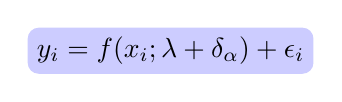
\begin{tikzpicture} \node [rounded corners,fill=blue!20] {
$y_i=f(x_i;\lambda+\delta_\alpha)+\epsilon_i$
};
\end{tikzpicture}
}
\vspace*{0.1cm}
\item Generalize parameter forms,\\
\vspace*{3mm}
\emph{Random field}\vspace*{-5mm}
\centerline{
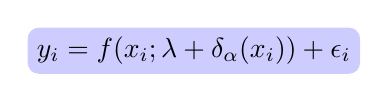
\begin{tikzpicture} \node [rounded corners,fill=blue!20] {
$y_i=f(x_i;\lambda+\delta_\alpha(x_i))+\epsilon_i$
};
\end{tikzpicture}
}
\vspace*{0.1cm}
\item More generally, explore additional parameterizations,\\
\vspace*{3mm}
\emph{Intrusive}\vspace*{-5mm}
\centerline{
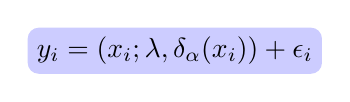
\begin{tikzpicture} \node [rounded corners,fill=blue!20] {
$y_i=\tf(x_i;\lambda,\delta_\alpha(x_i))+\epsilon_i$
};
\end{tikzpicture}
}
%\ebi

%\only<2>{
%\noindent\rule{12cm}{0.8pt}

%\small
%\bbi

\ei

\medskip

%}
\end{frame}

%==================================================================================
%==================================================================================
\begin{frame}[t]
\label{idea2}
\frametitle{Non-Intrusive Probabilistic Embedding}

Additive corrections $\delta_\alpha$ for input parameters $\lambda$\\
\medskip
\centerline{
% \begin{tikzpicture} \node [rounded corners,fill=blue!20] {
% $y_i=f(x_i;\lambda)+\delta(x_i)+\epsilon_i$
% };
% \end{tikzpicture}
%$\Longrightarrow$
%$\stackrel{\xrightarrow{\hspace*{2cm}}}{\textrm{\color{white}{a}}}$
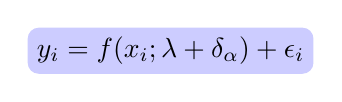
\begin{tikzpicture} \node [rounded corners,fill=blue!20] {
$y_i=f(x_i;\lambda+\delta_\alpha)+\epsilon_i$
};
\end{tikzpicture}
}

\medskip

\bi
\item Embed model error in specific submodel phenomenology
\bi
\item a modified transport or constitutive law
\item a modified formulation for a material property
\item turbulent model constants
\ei
\vspace*{0.4cm}
\item Allows placement of model error term in locations where key
modeling assumptions and approximations are made
\bi
\item as a correction or high-order term
\item as a possible alternate phenomenology
\ei
\vspace*{0.4cm}
%\item Explores the discrepancy on a given observable
\item Naturally preserves model structure and physical constraints
\item Disambiguates model/data errors

%\item Cons:
%\bi
%\item complex likelihood $p(y|\lambda)$ for general nonlinear
%$f(x,\lambda,\epsilon_m)$
%\ei
\ei
\end{frame}